\pagebreak
\subsection{The output from your first simulation}

After you have clicked on the \emph{Run Simulation} button (or pressed the function key F9) to run the simulation, the results from the simulation will have been written to disk. To view these results click on the \emph{Output} tab in the main window. There you will see the output from the simulation, this is visible in figure \ref{fig:output}
\begin{figure}[H]
\centering
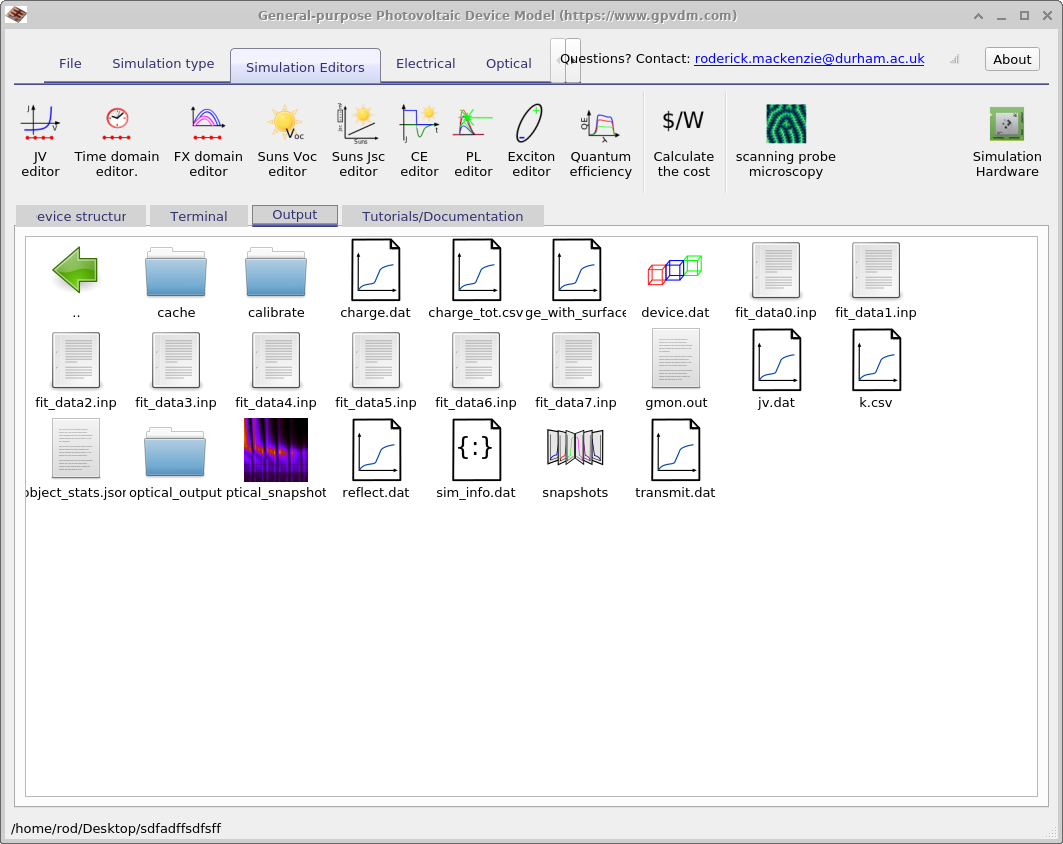
\includegraphics[width=0.6\textwidth,height=0.5\textwidth]{./images/running/output.png}
\caption{The \emph{Output} tab this is just like windows file explorer, you can explore the simulation directory tree.}
\label{fig:output}
\end{figure}


Key files the simulation produces are listed in the table below:

\begin{table}[H]
\begin{center}
\begin{tabular}{ |c|c|c| } 
 \hline
	File name 			& 	Description  \\ 
 \hline
	$jv.dat$ 			&	Current v.s. voltage curve \\ 
	$charge.csv$ 		&	Voltage v.s. charge density curve\\ 
	$device.dat$ 		&	The 3D device model\\ 
	$fit\_data*.inp$ 	&	Experimental data for this device.\\
	$k.csv$ 			&	Voltage v.s. Recombination constant k\\ 
	$reflect.csv$ 		&	Optical reflection from device\\ 
	$transmit.csv$ 		&	Optical transition through device\\ 
	$snapshots$ 		&	Electrical snapshots see \ref{sec:snapshots}\\
	$optical\_snapshots$&	Optical snapshots see \ref{sec:snapshotsoptical} \\
	$sim\_info.dat$ 	&	Calculated $V_{oc}$, $J_{sc}$ etc.. see \ref{sec:siminfo}   \\
	$cache$ 			&	Cache see \ref{sec:cache}  \\
 \hline
\end{tabular}
\caption{Files produced by the JV simulation}
\label{fig:output}
\end{center}
\end{table}

Try opening $jv.dat$. This is a plot of the voltage applied to the solar cell against the current generated by the device.  These curves are also sometimes called the \emph{characteristic diode curve}, we can tell a lot about the solar cell's performance by looking at these curves.  Hit the 'g' key to bring up a grid.

\begin{figure}[H]
\centering
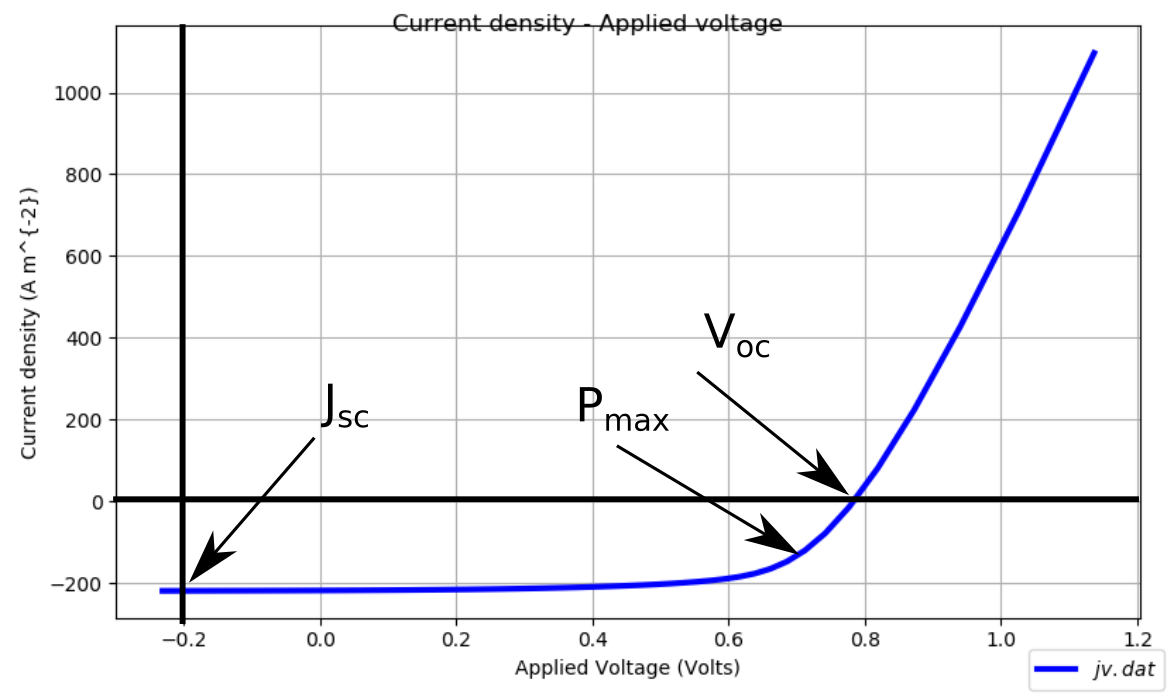
\includegraphics[width=0.6\textwidth]{./images/running/jv_curve.png}
\caption{The output tab}
\label{fig:jv_curve}
\end{figure}


Now try opening up the file $sim\_info.dat$, this file displays information on the performance of the solar cell, such as the Open Circuit Voltage ($V_{oc}$ - the maximum Voltage the solar cell can produce when iluminated), efficiency ($\eta$ - the efficiency of the cell) , and short circuit current ($J_{sc}$ - the maximum current the cell can produce when it is illuminated).  Figure \ref{fig:jv_curve}, shows where you can find these values on the JV curve.  The $sim\_info.dat$ file contains a lot of other parameters, these are described in detail in section \ref{sec:siminfo}.

\vspace*{\fill}
\fbox{
\parbox{0.9\textwidth}{
\color{blue} Question \addtocounter{question}{1}\thequestion: What is the $J_{sc}$, $V_{oc}$ and Fill Factor (FF) of this solar cell?  How do these number compare to a typical Silicon solar cell? (Use the internet to find typical values for a Silicon solar cell.)
}\par
}


